\documentclass[document,border=0pt]{standalone}

\usepackage{tikz}
\usepackage{color}
\usetikzlibrary{decorations.pathreplacing}

\begin{document}
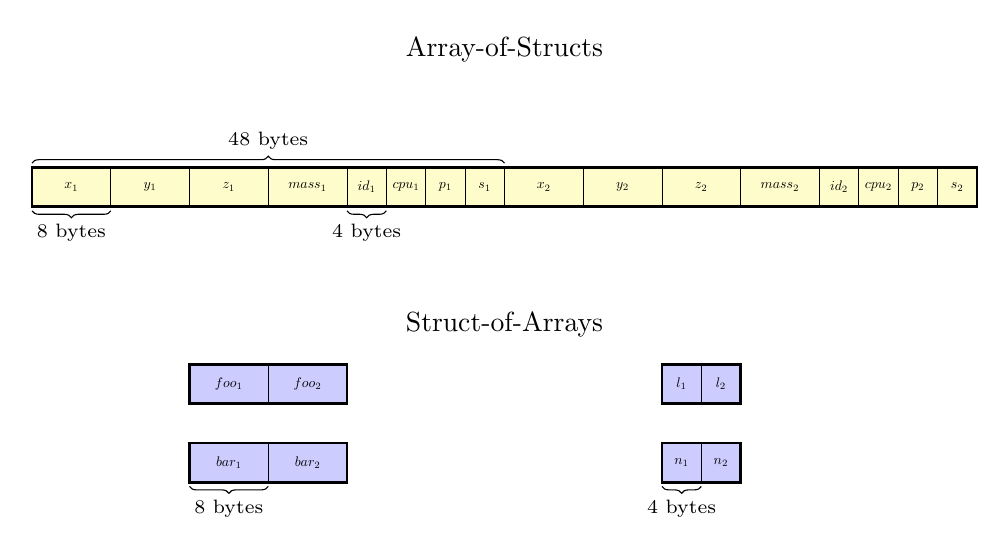
\begin{tikzpicture}

\draw (6.0, 7.5) node [scale=1.0]{Array-of-Structs};

\draw[black, line width=1, fill=yellow!20!white] (0,5.5) rectangle (12, 6.0);
\draw[step=1.0, black, line width=0.25] (0, 5.5) grid (4,  6.0);
\draw[step=0.5, black, line width=0.25] (4, 5.5) grid (6,  6.0);
\draw[step=1.0, black, line width=0.25] (6, 5.5) grid (10, 6.0);
\draw[step=0.5, black, line width=0.25] (10,5.5) grid (12, 6.0);
\draw (0.5,5.75) node [scale=0.5]{$x_1$};
\draw (1.5,5.75) node [scale=0.5]{$y_1$};
\draw (2.5,5.75) node [scale=0.5]{$z_1$};
\draw (3.5,5.75) node [scale=0.5]{$mass_1$};

\draw (4.25,5.75) node [scale=0.5]{$id_1$};
\draw (4.75,5.75) node [scale=0.5]{$cpu_1$};
\draw (5.25,5.75) node [scale=0.5]{$p_1$};
\draw (5.75,5.75) node [scale=0.5]{$s_1$};

\draw (6.5,5.75) node [scale=0.5]{$x_2$};
\draw (7.5,5.75) node [scale=0.5]{$y_2$};
\draw (8.5,5.75) node [scale=0.5]{$z_2$};
\draw (9.5,5.75) node [scale=0.5]{$mass_2$};

\draw (10.25,5.75) node [scale=0.5]{$id_2$};
\draw (10.75,5.75) node [scale=0.5]{$cpu_2$};
\draw (11.25,5.75) node [scale=0.5]{$p_2$};
\draw (11.75,5.75) node [scale=0.5]{$s_2$};

\draw (6.0,4.0) node [scale=1.0]{Struct-of-Arrays};

\draw[black, line width=1, fill=blue!20!white] (2,3) rectangle (4, 3.5);
\draw[step=1, black, line width=0.25] (2,3) grid (4, 3.5);
\draw (2.5,3.25) node [scale=0.5]{$foo_1$};
\draw (3.5,3.25) node [scale=0.5]{$foo_2$};

\draw[black, line width=1, fill=blue!20!white] (2,2) rectangle (4, 2.5);
\draw[step=1, black, line width=0.25] (2,2) grid (4, 2.5);
\draw (2.5,2.25) node [scale=0.5]{$bar_1$};
\draw (3.5,2.25) node [scale=0.5]{$bar_2$};

\draw[black, line width=1, fill=blue!20!white] (8,3) rectangle (9, 3.5);
\draw[step=0.5, black, line width=0.25] (8,3) grid (9, 3.5);
\draw (8.25,3.25) node [scale=0.5]{$l_1$};
\draw (8.75,3.25) node [scale=0.5]{$l_2$};

\draw[black, line width=1, fill=blue!20!white] (8, 2) rectangle (9, 2.5);
\draw[step=0.5, black, line width=0.25] (8, 2) grid (9, 2.5);
\draw (8.25,2.25) node [scale=0.5]{$n_1$};
\draw (8.75,2.25) node [scale=0.5]{$n_2$};

\draw [decorate, decoration={brace}, yshift=1.5]
(0.0, 6.0) -- (6.0, 6.0) node [black,midway,yshift=8.0]
{\scriptsize 48 bytes};

\draw [decorate,decoration={brace}, yshift=-1.5]
(1.0, 5.5) --  (0.0, 5.5) node [black,midway,yshift=-8.0]
{\scriptsize 8 bytes};

\draw [decorate,decoration={brace}, yshift=-1.5]
(4.5, 5.5) -- (4.0, 5.5) node [black,midway,yshift=-8.0]
{\scriptsize 4 bytes};

\draw [decorate,decoration={brace}, yshift=-1.5]
(3.0, 2) --  (2.0, 2) node [black,midway,yshift=-8.0]
{\scriptsize 8 bytes};

\draw [decorate,decoration={brace}, yshift=-1.5]
(8.5, 2) -- (8.0, 2) node [black,midway,yshift=-8.0]
{\scriptsize 4 bytes};

\end{tikzpicture}
\end{document}
